\documentclass{VUMIFPSkursinis}
\usepackage{algorithmicx}
\usepackage{algorithm}
\usepackage{algpseudocode}
\usepackage{amsfonts}
\usepackage{amsmath}
\usepackage{bm}
\usepackage{caption}
\usepackage{color}
\usepackage{float}
\usepackage{graphicx}
\usepackage{listings}
\usepackage{subfig}
\usepackage{wrapfig}

\newfontfamily\collfont[Path=./Palemonas-2.1/]{Palem-nm.ttf}
% Titulinio aprašas
\university{Vilniaus universitetas}
\faculty{Matematikos ir informatikos fakultetas}
% \institute{Informatikos institutas}  % Užkomentavus šią eilutę - institutas neįtraukiamas į titulinį
\department{Programų sistemų studijų programa}
\papertype{Kursinis darbas}
\title{Automatinis paukščių ant pastatų aptikimas ir atbaidymas lazeriu}
\titleineng{Automatic detection and deterrence of birds on buildings using a laser}
\status{4 kurso 1 grupės studentas}
\author{Tautvilis Savickas}
\supervisor{Prof. Dr. Aistis Raudys}
\date{Vilnius – \the\year}

% Nustatymai
  % Pakeisti teksto šriftą į Palemonas (turi būti įdiegtas sistemoje)
\bibliography{bibliografija}

\begin{document}
\maketitle

\tableofcontents

\sectionnonum{Įvadas}

Paukščių būriai sukelia daug žalos ūkiams bei miestams. Ūkininkai patyria didelę ekonominę žalą, kadangi paukščiai yra sudėtingi ir  mobilus kenkėjai - jie sunaikiną derlių \cite{refId0} ir platina ligas, kaip paukščių gripas. Miestuose paplitę paukščiai, kaip miesto balandžiai (Columba livia domestica) ar tikrieji varnėnai (Sturnus), daro didelę žalą savo išmatomis. Kadangi jie peri ant miesto pastatų, jų išmatos kaupiasi ir nėra dažnai valomos \ref{img:bird_poop} pav., todėl tampą skirtingų ligų šaltiniu. Jungtinėse Amerikos Valstijose invaziniai paukščiai sukėlė 1,1 milijardo JAV dolerių žalos \cite{article}. Taip pat balandžių išmatos yra labai rūgštingos ir gali padaryti žalą metalams bei mūriniams objektams, pavyzdžiui: mašinos, pastatai, paminklai. \cite{ahmed2021effect, shrestha2022conservation}.

\begin{figure}[H]
    \centering
    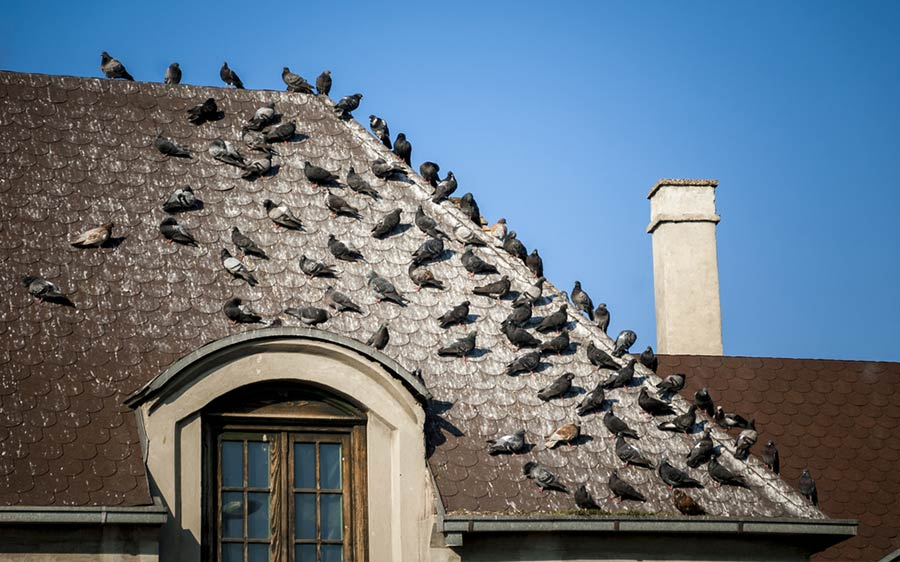
\includegraphics[scale=0.5]{img/bird_poop_on_roof.png}
    \caption{Balandžių pulko padaryta žala stogui.}
    \label{img:bird_poop}
\end{figure}

Paukščių atbaidymui yra naudojama daug skirtingų būdų, priklausančių nuo erdvės, kurioje reikia juo baidyti. Vaisių ūkininkai labai ilgą laiką naudoją tinklus, kad uždengtų medžius nuo kenkėjų, taip pat yra garsinės atbaidymo priemonės, tačiau jos veikia tame pačiame dažnyje, kuri žmonės gali girdėti ir sukelia daug nepatogumo. Oro uostuose dideli pavojų kelia skraidantis paukščiai. Paskaičiuota, kad globaliai per metus paukščių padaroma žala yra 1,2 milijardo JAV dolerių \cite{allan2000costs}. Bandant atbaidyti juos oro uostose yra naudojami sakalai-robotai \cite{robird}, tai maži, skraidantis lėktuvai, kurių korpusas padarytas, kad atvaizduotų sakalą. Taip pat, jis skraidydamas imituoja sakalų leidžiamus garsus ir plasnoja sparnais, taip gąsdindamas paukščius, kad šalia yra plėšrūnas. Miestuose populiariausias būdas atbaidyti paukščius yra spygliai \ref{img:bird_spikes} pav. Jie yra statomi ant pastogių, stogų, ar bet kur kitur, kur nėra pageidaujami paukščiai. Jų patrauklumas yra tai, kad jie yra efektyvus \cite{bird_spike}. Tačiau jų kainą yra didelė, greitai susidėvi jei nėra tinkamai prižiūrimi bei kelią grėsmę paukščiams. 

\begin{figure}[H]
    \centering
    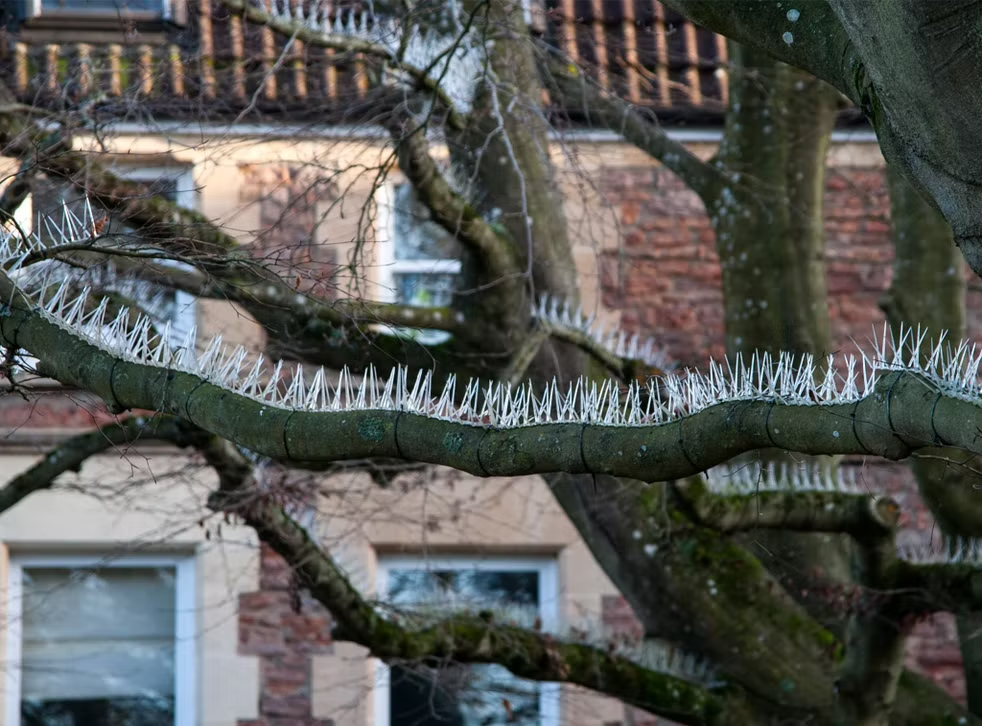
\includegraphics[scale=0.3]{img/bird_spikes.png}
    \caption{Paukščių atbaidymo spygliai.}
    \label{img:bird_spikes}
\end{figure}

Vienas iš gausiai paplitusių būdų atbaidyti paukščius, kuris tinkamas daugumai atvejų yra lazeriai. 1970-aisiais metais buvo pradėtas naudotas, kad apsaugotu lėktuvus nuo susidūrimo su paukščiais. Vėliau, lazeriai pradėti naudoti ir plačiau: ūkiuose, naftos platformose. JAV kukurūzų ūkininku laukuose be lazerinių atbaidymo prietaisų žala svyravo tarp 40\% ir 100\%, tačiau naudojant lazerius - sumažėjo iki 5\% \cite{brown2017laser}.

Šio darbo tikslas yra sukurti programinį sprendimą aptikti paukščius esančius ant pastatų ir simuliuoti lazerio judėjimo trajektoriją norint atbaidyti juos. Kuriamas sprendimas neturėtų kenkti paukščiams, o tik juos atbaidyti. Sprendimui įgyvendinti reikės 

Šio darbo tikslas yra surasti geriausiai veikianti dirbtinio intelekto modelį, kuris tinkamai aptiktų paukščius ant stogų ir apskaičiuotų lazerio švietimo trajektoriją taip, kad paukščiai nebūtų sužeisti. Darbe bus tiriama, koks yra tinkamiausias objektų aptikimo algoritmas, kaip duomenis įtakoja modelio veikimą ir lazerio judėjimas su atstumo įvertinimu.

Iškelti uždaviniai:
\begin{enumerate}
    \item Išanalizuoti esamus objektų aptikimo modelius;
    \item Sukurti duomenų rinkinį;
    \item Parinkti tinkamiausią objektų aptikimo modelį;
    \item Ištirti kaip objektų aptikimo modelis veikia su sukurtu ir jau esamais duomenų rinkiniais;
    \item 
\end{enumerate}



\section{Medžiagos darbo tema dėstymo skyriai}
Medžiagos darbo tema dėstymo skyriuose pateikiamos nagrinėjamos temos detalės:
pradinė medžiaga, jos analizės ir apdorojimo metodai, sprendimų įgyvendinimas,
gautų rezultatų apibendrinimas. Šios dalies turinys labai priklauso nuo darbo
temos. Skyriai gali turėti poskyrius ir smulkesnes sudėtines dalis, kaip
punktus ir papunkčius.

Medžiaga turi būti dėstoma aiškiai, pateikiant argumentus. Tekstas dėstomas
trečiuoju asmeniu, t.y. rašoma ne „aš manau“, bet „autorius mano“, „autoriaus
nuomone“. Reikėtų vengti informacijos nesuteikiančių frazių, pvz., „...kaip jau
buvo minėta...“, „...kaip visiems žinoma...“ ir pan., vengti grožinės literatūros
ar publicistinio stiliaus, gausių metaforų ar panašių meninės išraiškos
priemonių.

\subsection{Poskyris}
Citavimo pavyzdžiai: cituojamas vienas šaltinis

\subsubsection{Skirsnis}
\subsubsubsection{Straipsnis}
\subsubsection{Skirsnis}
\section{Skyrius}
\subsection{Poskyris}
\subsection{Poskyris}

\sectionnonum{Rezultatai ir išvados}
Rezultatų ir išvadų dalyje turi būti aiškiai išdėstomi pagrindiniai darbo
rezultatai (kažkas išanalizuota, kažkas sukurta, kažkas įdiegta) ir pateikiamos
išvados (daromi nagrinėtų problemų sprendimo metodų palyginimai, teikiamos
rekomendacijos, akcentuojamos naujovės).

\printbibliography[heading=bibintoc]  % Šaltinių sąraše nurodoma panaudota
% literatūra, kitokie šaltiniai. Abėcėlės tvarka išdėstomi darbe panaudotų
% (cituotų, perfrazuotų ar bent paminėtų) mokslo leidinių, kitokių publikacijų
% bibliografiniai aprašai.  Šaltinių sąrašas spausdinamas iš naujo puslapio.
% Aprašai pateikiami netransliteruoti. Šaltinių sąraše negali būti tokių
% šaltinių, kurie nebuvo paminėti tekste.

% \sectionnonum{Sąvokų apibrėžimai}
\sectionnonum{Santrumpos}
Sąvokų apibrėžimai ir santrumpų sąrašas sudaromas tada, kai darbo tekste
vartojami specialūs paaiškinimo reikalaujantys terminai ir rečiau sutinkamos
santrumpos.

\appendix  % Priedai
% Prieduose gali būti pateikiama pagalbinė, ypač darbo autoriaus savarankiškai
% parengta, medžiaga. Savarankiški priedai gali būti pateikiami ir
% kompaktiniame diske. Priedai taip pat numeruojami ir vadinami. Darbo tekstas
% su priedais susiejamas nuorodomis.

\section{Neuroninio tinklo struktūra}
\begin{figure}[H]
    \centering
    \includegraphics[scale=0.5]{img/MLP}
    \caption{Paveikslėlio pavyzdys}
    \label{img:mlp}
\end{figure}


\section{Eksperimentinio palyginimo rezultatai}
% tablesgenerator.com - converts calculators (e.g. excel) tables to LaTeX
\begin{table}[H]\footnotesize
  \centering
  \caption{Lentelės pavyzdys}
  {\begin{tabular}{|l|c|c|} \hline
    Algoritmas & $\bar{x}$ & $\sigma^{2}$ \\
    \hline
    Algoritmas A  & 1.6335    & 0.5584       \\
    Algoritmas B  & 1.7395    & 0.5647       \\
    \hline
  \end{tabular}}
  \label{tab:table example}
\end{table}

\end{document}
